\subsection{Modularity and comparison to purely symbolic representations}\label{ssec:set_exp}


\begin{wrapfigure}{R}{0.25\textwidth}
	\vskip-5pt
	\begin{tabular}{c}
		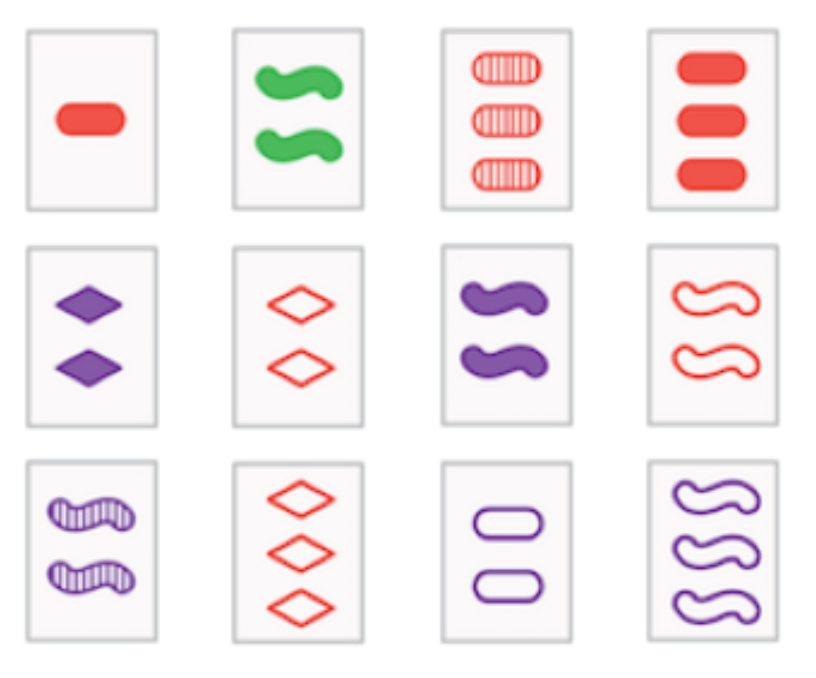
\includegraphics[width=.25\textwidth]{figures/set_example}\\[-5pt]
	\end{tabular}
	\caption{\footnotesize The SET game}
\end{wrapfigure}
SET is a relatively straightforward but challenging cognitive task that engages reasoning faculties in a deliberative
, attentionally directed manner, requiring several levels of abstraction over sensory embeddings. Players are
presented with 12 cards, each of which contains figures that vary along four dimensions (color, number, pattern, and
shape) and they must find subsets of three cards which obey a deceptively simple rule: along each dimension, all cards in a SET must either have the same or unique values.
% JDC: DO FIGURES NEED TO BE NUMBERED?
For example, in the figure to the right, the cards with two solid blue/purple diamonds, two striped blue squiggles, and two open blue oblongs form a SET: same color, same number, different patterns, different shapes.

To simulate the task of deciding if a triple forms a SET, we first train a convolutional neural network to process the color images of the cards (a full deck includes 81 cards). The CNN is trained to predict the attribute of
each card, as a multi-label classification, and then an embedding of dimension $d=32$ of 
each card is obtained. This embedding layer uses an \MLP{} to map the convolutional feature maps into a distributed
representation. Next, we train Abstractors separately for each of the four attributes to learn same/different
relations, where the task is to decide if an input pair of cards is the same or different for that attribute. 
We then use the query and key mappings $W_Q$ and $W_K$ learned for these relations to initialize the relations
in a multi-head Abstractor. The Abstractor is then trained on a dataset of triples of cards, half of which form a SET. 

This is compared to a baseline symbolic model where, instead of images, the input is a vector with 12 bits,
explicitly encoding the relations. That is, for each of the four attributes, a binary symbol is computed for each pair of three input cards---1 if the pair is the same in that attribute, and 0 otherwise. A two-layer MLP is then trained to decide if the triple forms a SET. The MLP using the symbolic representation can be considered as a lower bound on the performance achievable by the Abstractor. This comparison shows that the Abstractor is able to solve a task using relations learned in other tasks (modularity), with a sample efficiency that is not far from that obtained
with purely symbolic, noise-free encodings of the relevant relations. %We note that this uses a simple Abstractor configuration, without self-attention.

% JDC: I REALIZE WE ARE TIGHT ON SPACE, BUT IF THERE IS ROOM, COULD ADD THE FOLLOWING, OR A SHORTENED FORM OF
This subtask suggests how Abstractors might be viewed as an intermediate between strong ``nativist'' approaches that assume a pre-existing foundation of symbolic primitives and purely ``empiricist'' approaches that assume
similar capabilities can emerge simply from processing large amounts of data~\cite{lake2015}.
%can be achieved simply by the application of general purpose learning algorithms to large
%amounts of data -- showing how the latter, agumented with simple architectural inductive biases and trained using
%plausible and practical forms of curricular learninng both to generate genuinely symbolic representations, and use these to achieve the flexibilty and efficiency characteristic of human reasoning.
